\documentclass[10pt]{beamer}

%STANDARD PREAMBLE
%https://tex.stackexchange.com/questions/68821/is-it-possible-to-create-a-latex-preamble-header
\usepackage{/Users/mwojno01/Research/Learning/latex_preamble/beamer_preamble}

%
%% ALLOW FOR ITEMIZE ENVIRONMENTS WITH NO PRECEDING
% SPACING, IF DESIRED
% Reference: https://tex.stackexchange.com/questions/86054/how-to-remove-the-whitespace-before-itemize-enumerate
%\usepackage{enumitem}% http://ctan.org/pkg/enumitem 
\usepackage{paralist}

% RANDOM VARIABLE
\newcommand{\x}{X}
\newcommand{\y}{Y}


\title{Bayesian Inference: Conjugate Models}

\begin{document}

\maketitle






\begin{frame}{Bayes' Rule}
\footnotesize

\begin{sblock}{Bayes' Rule}
\[ \underset{posterior}{p(\theta|x)} = \df{ \underset{likelihood}{p(x|\theta)} \quad  \underset{prior}{p(\theta)} }{ \underset{evidence}{p(x)}}  = \dfrac{p(x | \theta) p(\theta)}{\int p(x | \theta) p(\theta) \, d\theta}  \]
\end{sblock}

\begin{sblock}{Posterior}
The posterior distribution is proportional to the prior times the likelihood:
\[p(\theta | x) \propto p(x | \theta) p(\theta)\]

The posterior distribution \textit{is a distribution} over $\theta$.

\end{sblock}

\begin{sblock}{Evidence}
The evidence, or \textit{marginal likelihood}, can be used for model comparison.
\end{sblock}

\end{frame}


%%%%%%%%%

\begin{frame}{Example: Beta-bernoulli model}
Sometimes, we can compute the posterior distribution by hand, given prior and likelihood.

\begin{sblock}{Setup: flipping a coin}
Probability that it lands heads is (unknown) $\theta$. \\
Prior probability over $\theta$ assumed to follow a $Beta(3,3)$ distribution:
$$ p(\theta) = \frac{\theta^{3-1}(1-\theta)^{3-1}}{B(3,3)}$$
Note: $\theta \sim Beta(a, b)$ means $p(\theta) \propto \theta^{a-1}(1-\theta)^{b-1}$\\
Will collect data by flipping coin once. Likelihood of observing heads ($x=1$) or tails ($x=0$) is given by a Bernoulli distribution:
$$p(x | \theta) = \theta^x(1-\theta)^{1-x} $$.
\end{sblock}


\end{frame}

\begin{frame}{Example: Beta-Bernoulli model}

\begin{sblock}{Setup: flipping a coin}
Probability that it lands heads is (unknown) $\theta$. \\
Prior probability over $\theta$ assumed to follow a $Beta(3,3)$ distribution:
$$ p(\theta) = \frac{\theta^{3-1}(1-\theta)^{3-1}}{B(3,3)}$$
{\tiny Note: $\theta \sim Beta(a, b)$ means $p(\theta) = \frac{1}{B(a,b)}\theta^{a-1}(1-\theta)^{b-1}$, where $B(a,b):= \frac{\Gamma(a) \Gamma(b)}{\Gamma(a+b)}.$}
\vfill 
Will collect data by flipping coin once. Likelihood of observing heads ($x=1$) or tails ($x=0$) is given by a Bernoulli distribution:
$$p(x | \theta) = \theta^x(1-\theta)^{1-x} $$.
\end{sblock}
\begin{sblock}{Computing the posterior after observing x=1}
$$p(\theta| x) \propto p(x | \theta) p(\theta) = \theta^1(1-\theta)^{0}  \theta^{2}(1-\theta)^{2}  = \theta^3 (1-\theta)^2 \implies \theta | x \sim Beta(4,3)$$
\end{sblock}

\end{frame}

%%%%%%%%%%%%%%%

\begin{frame}{Conjugacy}

\begin{sblock}{The idea}
We have conjugacy when the prior and the posterior distributions are in the same family (e.g. in the previous example, the prior and posterior are beta distributions).
\end{sblock}

\begin{sblock}{Definition}
Conjugacy can be defined as follows \cite{gelman2013bayesian}. If $\mathcal{F}$ is a class of sampling distributions and $\mathcal{P}$ is a class of prior distributions for $\theta$, then the class $\mathcal{P}$ is \textit{conjugate} for $\mathcal{F}$ if
\[  p(\theta \cond y ) \in \mathcal{P} \; \text{for all} \; p(\cdot \cond \theta) \in \mathcal{F} \; \text{and} \; p(\cdot) \in \mathcal{P} \]
\end{sblock}

\bottomtext{Technical note: the condition trivially holds if $\mathcal{P}$ is taken to be the space of all probability distributions!}
\end{frame}


%%%%%%%%%%%%%%

\begin{frame}{Posterior predictive distribution}

\begin{sblock}{Given}

$p(\theta | x)$ - posterior \\
$p(\theta)$ - prior \\
$p(x | \theta)$ - likelihood

\end{sblock}

\begin{sblock}{Posterior predictive distribution}

Consider the probability of new data $x'$. Posterior predictive distribution is:

$p(x' | x) = \int p(x', \theta | x) \, d\theta = \int p(x' | \theta, x) p(\theta |x) \, d\theta = \int p(x' | \theta) p(\theta | x) \, d\theta$

Incorporates the knowledge and uncertainty about $\theta$ that we still had after seeing data $x$.

\end{sblock}

\end{frame}

\begin{frame}{Another example: The Gamma-Poisson model}

Some measurements, such as a person's number of children or number of friends, have values that are whole numbers.    Perhaps the simplest probability model on whole numbers is the Poisson model.

\begin{minipage}{.48\textwidth}
\begin{itemize}
\item \textbf{Sample}: $X$ the observed number.
\item \textbf{Sample space}: $\mathcal{X} = \set{0,1,2,...}$
\item \textbf{Density:}
\begin{equation}
p(x \cond \lambda) = \df{\lambda^x e^{-\lambda}}{x!} 
\label{eqn:poisson_density}	 
\end{equation}

 \item \textbf{Parameter:} $\lambda = \E[X]$
\item \textbf{Parameter space}: $\lambda \in (0,\infty)$ 

\end{itemize}
\end{minipage} \hfill 
\begin{minipage}{.48\textwidth}

\begin{center}
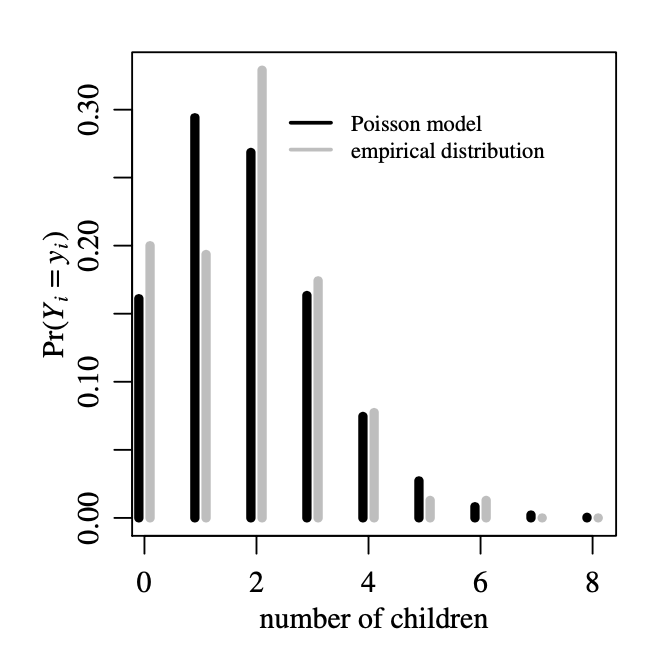
\includegraphics[width=\textwidth]{images/hoff_poisson}	
\scriptsize A Poisson distribution with mean $1.83$, along with the empirical distribution of the number of children of women of age 40 from the GSS during the 1990's
\end{center}

\end{minipage} 


\end{frame}


\begin{frame}{The Gamma-Poisson model}

The Gamma distribution is a conjugate prior for the Poisson likelihood.  Can you show this?	 \pause 

Given observations $\+x = (x_1, ..., x_n)$, we have

\begin{align*}
p(\lambda) & \propto \lambda^{\bluemathbox{\alpha}-1} \exp \big\{-\greenmathbox{\beta} \lambda \big\}  \\
p(\+x \cond \lambda) & \stackrel{iid}{=} \ds\prod_{i=1}^n p(x_i \cond \lambda) \\ & \stackrel{(Poisson)}\propto \lambda^{\bluemathbox{\sum_{i=1}^n x_i}} \exp \big\{-\greenmathbox{n} \lambda \big\}
\intertext{so}
p(\lambda \cond \+x) & \propto p(\+x \cond \lambda) p(\lambda) \\
&=  \lambda^{\bluemathbox{(\alpha + \sum_i x_i)}-1} \exp \big\{ -\greenmathbox{(\beta +n)}\lambda \big\} 
\end{align*}

\end{frame}

\begin{frame}{The Gamma-Poisson model}

That is, 
\begin{align*}
\lambda & \sim \text{Gamma} (\alpha, \beta)\\
x_i \cond \lambda & \iid \text{Poisson}(\lambda) \\
\implies \lambda \cond \+x &\sim \text{Gamma}(\alpha + \sum_{i=1}^n x_i, \beta + n)
\end{align*}

\end{frame}

\begin{frame}{Gamma-Poisson Model: Posterior Expectation}
Can you write the posterior expectation as a compromise between the prior expectation and sample mean {\tiny (like we did for the Beta-Bernoulli model)}?  \pause 

\begin{align*}
\E[\lambda] &= \df{\alpha}{\beta} && \tinytext{Gamma dist.} \\
\E[\lambda \cond \+x] &= \df{\alpha + \sum_{i=1}^n x_i}{\beta +n} && \tinytext{Gamma dist.} \\
&= \df{\beta}{\beta+n} \; \explaintermbrace{prior expectation}{\df{\alpha}{\beta}} \; +\; \df{n}{\beta+n} \;  \explaintermbrace{sample mean}{\df{\sum_{i=1}^n x_i}{n}}
\end{align*}

\textit{Interpretation?} \pause 
\begin{itemize}
	\item $\beta$: number of prior observations
	\item $\alpha$: sum of counts from $\beta$ prior observations
\end{itemize}

	
\end{frame}

\begin{frame}{Selecting a prior}

The previous slide gives us one way to specify the prior distribution: 

\begin{center}
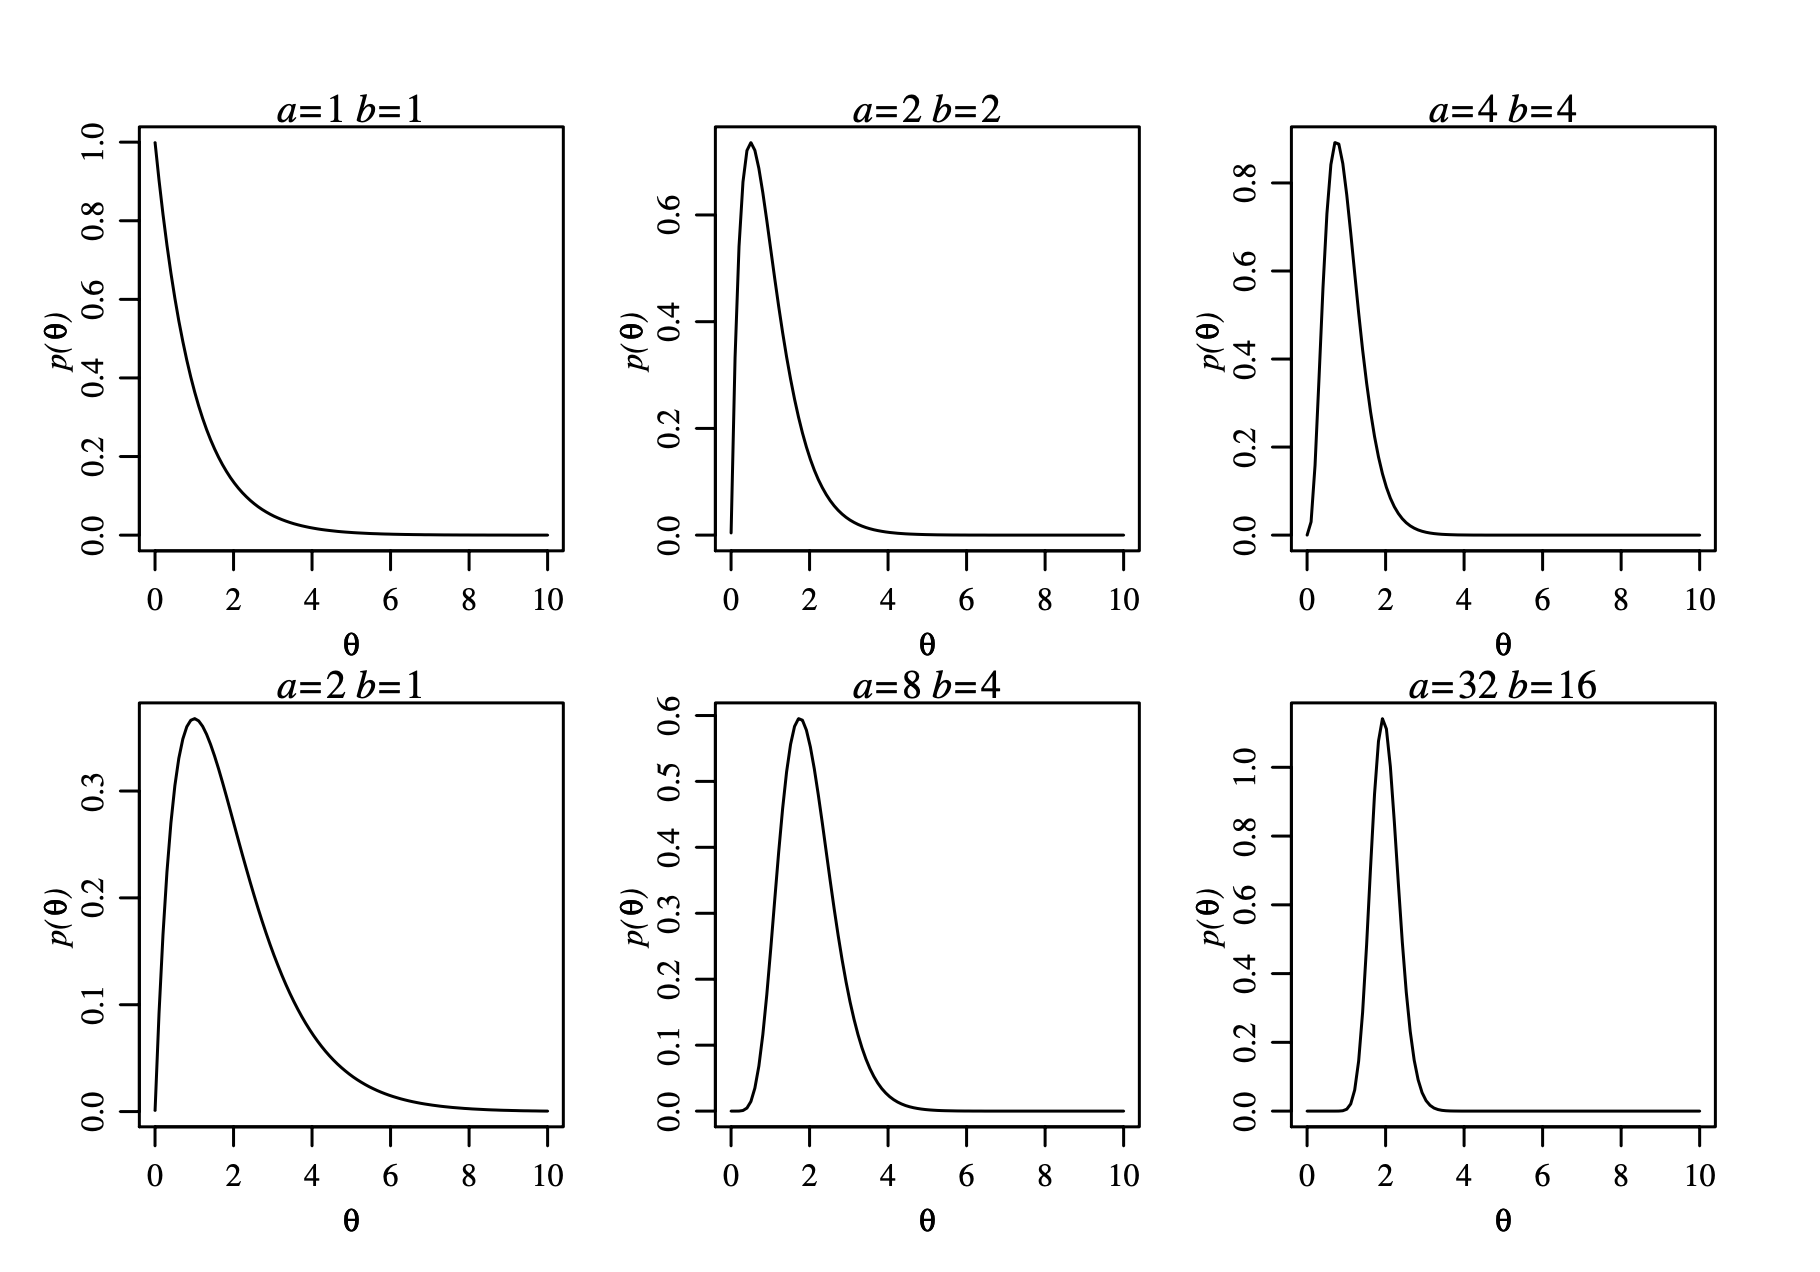
\includegraphics[width=.75\textwidth]{images/hoff_gamma}	
\end{center}

``My prior belief is that the average count in the population is $\frac{\alpha}{\beta}$, and I am as certain about this as if I had observed this in a sample of size $\beta$."
\end{frame}

\begin{frame}{Gamma-Poisson Model: Posterior Predictive}

The posterior predictive for the Gamma Poisson is given by 
\[ x_{\text{new}} \sim \text{NegativeBinomial}\bigg(\alpha', \df{1}{1+\beta'} \bigg) \]	
where $(\alpha', \beta')$ are the posterior parameters of the Gamma.
\vfill 
The Negative Binomial is a \textit{two-parameter} alternative to the Poisson model which provides a flexible model of count data {\tiny (e.g., it can handle overdispersion)} 
\end{frame}






%%%%%%%%%%%%%%%

\begin{frame}{Tractability notes}

Generally, computing the posterior distribution is much harder than in this example!
\vfill
Consider the denominator in $ p(\theta | x) = \dfrac{p(x | \theta) p(\theta)}{\int p(x | \theta) p(\theta)} \, d\theta $  - integrals are hard 
\vfill
In nonconjugate examples, we need approaches to work with the posterior distribution when we cannot calculate it directly. Stay tuned!

\end{frame}

%%%%%%%%%%%%%%%
\begin{frame}{Exponential families}

The Bernoulli and the Poisson distributions are both \blue{\href{https://github.com/mikewojnowicz/exponential_family/blob/297dde8bf81b09544b66f3b80324db44bc601358/exponential_family.pdf}{exponential families.}}
 
\metroset{block=fill}
\begin{block}{Exponential family}
An \textit{exponential family} is a set of probability distributions whose probability density functions have the following form
\begin{align*}
\label{eqn:exponential_family}
 p(x \cond \theta) = h(x) \exp \{ \eta(\theta)^T t(x) - a(\theta)\} 
\end{align*}
where we refer to $h$ as the base measure, $\eta$ as the natural parameter, $t$ as the sufficient statistics, and $a$ as the log normalizer. 
\end{block}

\pause 
\begin{sblock}{Why do we care?}
 \pause 
\begin{itemize}
\item \textit{Any} probability model in the exponential family has a \blue{\href{https://en.wikipedia.org/wiki/Conjugate_prior}{conjugate prior.}} \pause 
\item When the conjugate prior is used, you get the posterior and posterior predictive in \alert{closed form}! 
\end{itemize}
\end{sblock}

\end{frame}


%%%%%%%%%




%%%%%%%%%%%%%%%%







\end{document}